%==================================================================================================================================%
%============================================================= 第二章 预备知识 ====================================================%
%==================================================================================================================================%
\newpage
\chapter{预备知识} \label{Chap:SCFT_on_surface}
\subsection{网格}
在有限空间的构造中,我们需要通过网格来建立基函数,通过基函数来表示有限元空间,因此网格是建立有限元空间的核心结构,是实现数值离散方法的基础,我们需要对网格有一个大致的了解。

FEALPy的数据结构是用数组表示。

\begin{itemize}
	\item[$\bullet$] 三角形、四边形、四面体和六面体等网格,因为每个单元顶点的个
	数固定,因此可以用{\bf 节点坐标数组} node 和{\bf 节点间关系数组} cell 来表
	示,这是一种以{\bf 单元为中心的数据结构}。
	\item[$\bullet$] 其它的如{\bf 边数组} edge、{\bf 面数组} face 都可由 cell 生
	成。
	\item[$\bullet$] FEALPy 中把 node、edge、face 和 cell 统称为网格中的实体 entity。
	其中 cell 表示最高维的数组
	\item[$\bullet$] 在二维情形下,FEALPy 中的 edge 和 face 意义是相同的。
	\item[$\bullet$] FEALPy 中还有一种以{\bf 边中心的网格数据结构}, 称为{\bf 半边数
		据结构(Half-Edge data structure)},它具有更灵活和强大的网格表达能力。
\end{itemize}

以简单的网格来介绍上面的概念,和数据结构


Fealpy中已经实现的网格类
\begin{table}[H]
	\centering
	\begin{tabular}[c]{|c|c|}\hline
		IntervalMesh      & 区间网格        \\\hline
		TriangleMesh      & 三角形网格       \\\hline
		QuadrangleMesh    & 四边形网格       \\\hline
		TetrahedronMesh   & 四面体网格       \\\hline
		HexahedronMesh    & 六面体网格       \\\hline
		PolygonMesh       & 多边形网格       \\\hline
		PolyhedronMesh    & 多面体网格       \\\hline
		StructureQuadMesh & 结构四边形网格   \\\hline
		StructureHexMesh  & 结构六面体网格   \\\hline
		Tritree           & 三角形树结构网格 \\\hline
		Quadtree          & 四叉树           \\\hline
		OCtree            & 八叉树           \\\hline
		HalfEdgeMesh2d    & 二维半边网格     \\\hline
		HalfEdgeMesh3d    & 三维半边网格     \\\hline
	\end{tabular}
	\caption{FEALPy 中的网格类。}
\end{table}

在了解完实体的概念后,我们还需要了解不同实体间的关系,在fealpy里用ds来管理。
\begin{table}[H]
	\centering
	\begin{tabular}{|l|l|}\hline
		成员函数名 & 功能\\\hline
		cell2cell = mesh.ds.cell\_to\_cell(...) &单元与单元的邻接关系\\\hline
		cell2face = mesh.ds.cell\_to\_face(...) &单元与面的邻接关系\\\hline
		cell2edge = mesh.ds.cell\_to\_edge(...) &单元与边的邻接关系\\\hline
		cell2node = mesh.ds.cell\_to\_node(...) &单元与节点的邻接关系\\\hline
		face2cell = mesh.ds.face\_to\_cell(...) &面与单元的邻接关系\\\hline
		face2face = mesh.ds.face\_to\_face(...) &面与面的邻接关系\\\hline
		face2edge = mesh.ds.face\_to\_edge(...) &面与边的邻接关系\\\hline
		face2node = mesh.ds.face\_to\_node(...) &面与节点的邻接关系\\\hline
		edge2cell = mesh.ds.edge\_to\_cell(...) &边与单元的邻接关系\\\hline
		edge2face = mesh.ds.edge\_to\_face(...) &边与面的邻接关系\\\hline
		edge2edge = mesh.ds.edge\_to\_edge(...) &边与边的邻接关系\\\hline
		edge2node = mesh.ds.edge\_to\_node(...) &边与节点的邻接关系\\\hline
		node2cell = mesh.ds.node\_to\_cell(...) &节点与单元的邻接关\\\hline
		node2face = mesh.ds.node\_to\_face(...) &节点与面的邻接关系\\\hline
		node2edge = mesh.ds.node\_to\_edge(...) &节点与边的邻接关系\\\hline
		node2node = mesh.ds.node\_to\_node(...) &节点与节点的邻接关系\\\hline
	\end{tabular}
	\caption{网格拓扑数据成员 ds 的方法成员。} 
\end{table}

\section{数据结构}
\subsection{cell}
\begin{itemize}
	\item 每一行为一个单元,其中的数字为node的全局编号
	\item cell的编号顺序默认为逆时针
\end{itemize}
\subsection{edge}
\begin{itemize}
	\item 边界边的话,按两个端点看,左手边指向内部
	\item 内部边没有强制的顺序
\end{itemize}
\subsection{edge2cell}
edge2cell为边和单元的对应关系。以下图为列:
\begin{itemize}
	\item edge2cell的每一行对应的是edge的每一条边
	\item edge2cell前两列代表边左右相邻的单元号,若为边界边则两列数字一样
	\item edge2cell后两列代表边在对应单元(第三列对应第一列,第四列对应第二列)的边的局部编号
	\remark{点在单元中的局部编号为cell中所处的位置(从零开始)}
	\remark{边在单元中的局部编号为该边所对点的局部编号}
\end{itemize}

\begin{figure}[htbp]
	\begin{minipage}[t]{0.35\linewidth}
		\centering
		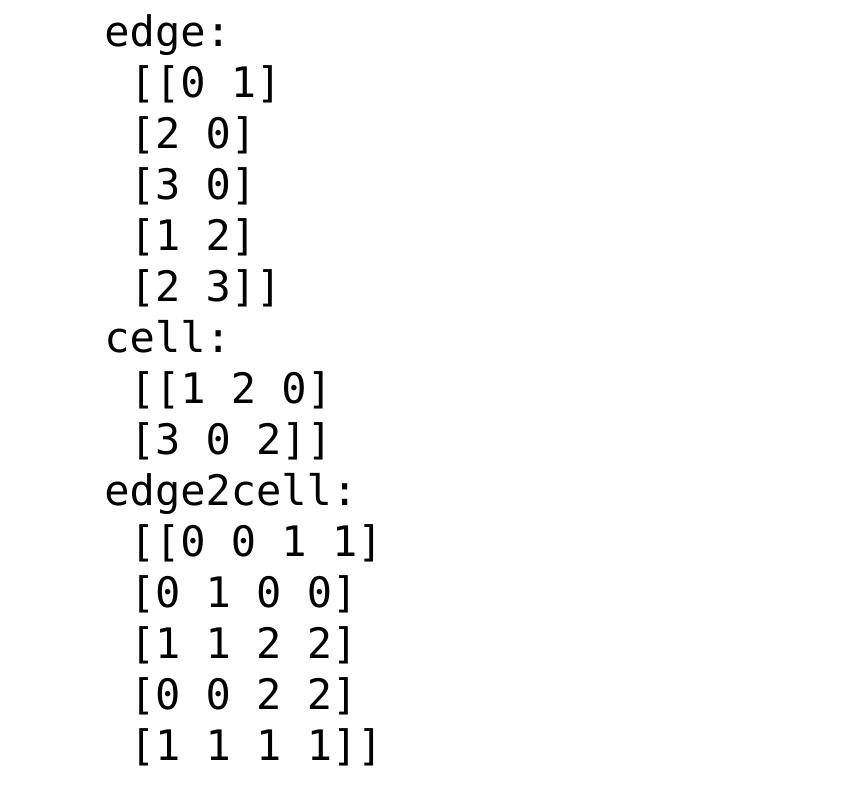
\includegraphics[scale=0.5]{figures/fealpy/edge2cell-0}
		\caption{}
	\end{minipage}%
	\hfill
	\begin{minipage}[t]{0.5\linewidth}
		\centering
		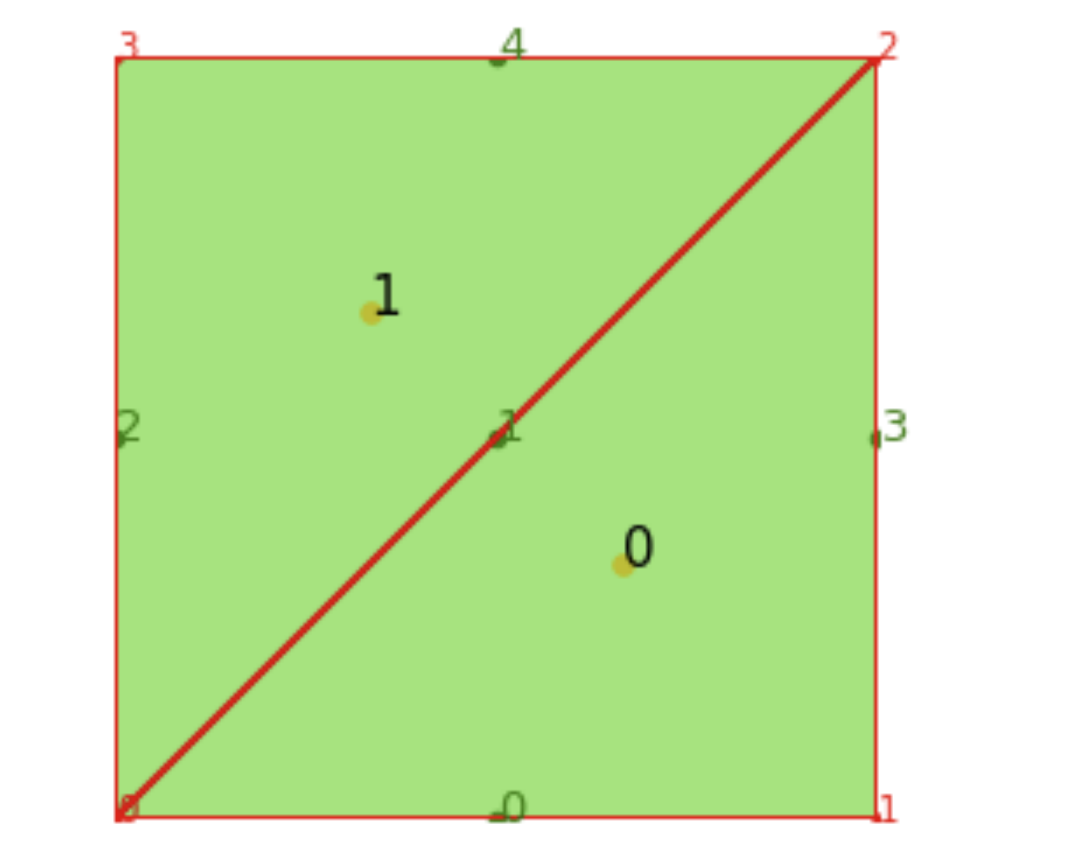
\includegraphics[scale=0.5]{figures/fealpy/edge2cell-1}
		\caption{}
	\end{minipage}
\end{figure}

\newpage
\section{模块}
\subsection{MeshFactory}
用于更有效率的生成各种各样的网格
\subsubsection{boxmesh2d}
其为MeshFactory所生成对象的一种方法,用来将方形区域进行结构网格的生成,所含参数有:
\begin{itemize}
	\item box:所要形成方形区域的长和宽的最大值和最小值
	\item nx:长所要进行的剖分段数
	\item ny:宽所要进行的破分段数
	\item meshtype:所有分网格的类型
\end{itemize}

\begin{figure}[htbp]
	\begin{minipage}[t]{0.35\linewidth}
		\centering
		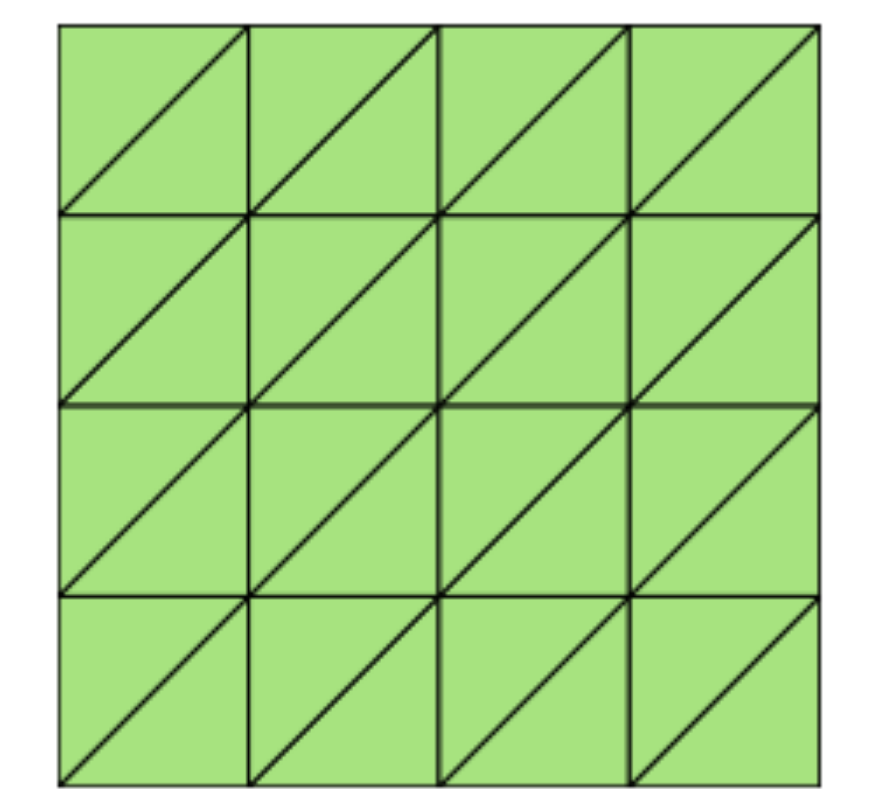
\includegraphics[scale=0.5]{figures/fealpy/boxmesh2d-tri}
		\caption*{box, nx=4, ny=4, meshtype='tri'}
	\end{minipage}%
	\hfill
	\begin{minipage}[t]{0.5\linewidth}
		\centering
		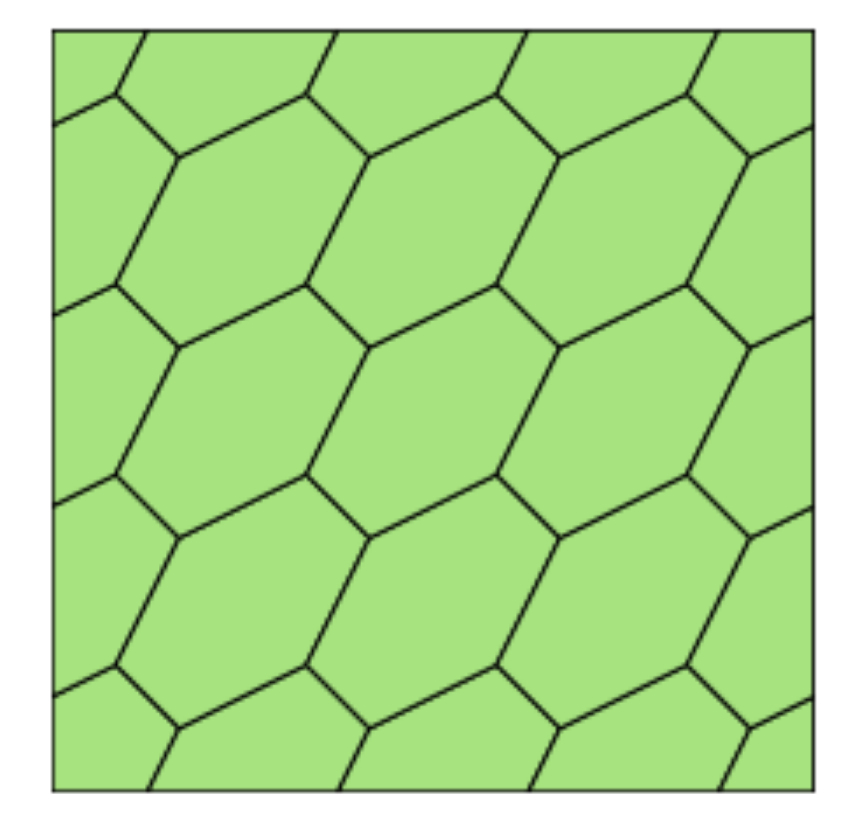
\includegraphics[scale=0.5]{figures/fealpy/boxmesh2d-poly}
		\caption*{box, nx=4, ny=4, meshtype='poly'}
	\end{minipage}
\end{figure}

\subsubsection{triangle}
其为MeshFactory所生成对象的一种方法,用来将方形区域进行非结构网格的生成,所含参数跟boxmesh2d一样,nx,ny换成h为网格的尺寸。

\subsubsection{special-boxmesh2d}
其为MeshFactory所生成对象的一种方法,用来将方形区域进行特殊结构网格的生成。